% Created 2017-10-28 Sat 22:36
\documentclass[a4paper]{article}
\usepackage[utf8]{inputenc}
\usepackage[T1]{fontenc}
\usepackage{fixltx2e}
\usepackage{graphicx}
\usepackage{longtable}
\usepackage{float}
\usepackage{wrapfig}
\usepackage{rotating}
\usepackage[normalem]{ulem}
\usepackage{amsmath}
\usepackage{textcomp}
\usepackage{marvosym}
\usepackage{wasysym}
\usepackage{amssymb}
\usepackage{hyperref}
\tolerance=1000
\usepackage{minted}
\usepackage[margin=0.8in]{geometry}
\usepackage{amssymb,amsmath}
\usepackage[nottoc,numbib]{tocbibind}
\usepackage{fancyhdr} %For headers and footers
\pagestyle{fancy} %For headers and footers
\usepackage{lastpage} %For getting page x of y
\usepackage{float} %Allows the figures to be positioned and formatted nicely
\restylefloat{figure} %and this command
\usepackage{hyperref}
\hypersetup{urlcolor=blue}
\usepackage{minted}
\setminted{frame=single,framesep=10pt}
\chead{}
\rhead{\today}
\cfoot{}
\rfoot{\thepage\ of \pageref{LastPage}}
\usepackage[parfill]{parskip}
\usepackage{subfig}
\hypersetup{colorlinks=true,linkcolor=black, citecolor=black}
\AtBeginEnvironment{minted}{%
\renewcommand{\fcolorbox}[4][]{#4}}
\usepackage{framed}
\author{Nathan Hughes (\href{mailto:nah31@aber.ac.uk}{nah26@aber.ac.uk})}
\date{\today}
\title{Assignment 1}
\hypersetup{
  pdfkeywords={},
  pdfsubject={},
  pdfcreator={Emacs 25.3.1 (Org mode 8.2.10)}}
\begin{document}

\maketitle
\vspace{2cm}

\begin{center}

\includegraphics[width=4cm]{./ruby.png}
\end{center}

\clearpage
\tableofcontents
\clearpage

\section{CSA Architecture}
\label{sec-1}
The Computer Science Alumni application aims to be relatively simple; it allows for users and posts 
to be created, held in a database and persist across sessions and users; This project was made 
following the specifications laid out in \cite{loftus17_requir_cs_alumn_applic}. 

It makes ample use of the Ruby on Rails framework, using generators to quickly template large sections
of code as well as a Model View Controller (Model-2 variant) to organise the overarching project.

The interaction and member variables of the two classes, User and Post can be
 seen in Fig.\ref{fig:userposts}.

\subsection{User}
\label{sec-1-1}
The User class exists in order to record the information of individuals using this web application.
We use the data provided here in order to link information made in the Posts class back to Users
where possible. 


\subsection{Post}
\label{sec-1-2}
Posts is a simple class which has three attributes "title", "body" and "email". These allow for simple
text based "broadcasts" to be made either anonymously or by a user, which is referenced by the "email"
attribute. If the given email of the post matches with any in our Users table, then we create the link
between the two.

\subsection{Routes}
\label{sec-1-3}
Part of this application is having a functioning routing table, as seen in  Listing.\ref{lst:routes}, 
this allows for the route '/' of our page to be a redirection to a static homepage. Additionally 
an extra line has been added to redirect 404 errors back to the home page.

\begin{listing}[H]
\begin{minted}[]{ruby}
Rails.application.routes.draw do
  resources :users
  resources :posts

  root 'static_pages#home'
  # Send errors to root
  get '*path' => redirect('/')
end
\end{minted}
\caption{\label{lst:routes}Routing}
\end{listing}

\subsection{Navigation}
\label{sec-1-4}
The CSA application provides a dynamic menu bar which (planned future functionality) changes the items
in the menu, based on the authentication/credentials of the logged in user. Admin checking can be seen
 in Listing.\ref{lst:navigation}

\begin{listing}[H]
\begin{minted}[]{ruby}
primary.item :home, 'Home', '/home', highlights_on: /(^\/$)|(^\/home$)/
primary.item :jobs, 'Jobs', '/jobs'
primary.item :profile, 'Profile', '/profile', if: Proc.new { is_admin? }
primary.item :users, 'Users', users_path, if: Proc.new { is_admin? }
primary.item :broadcasts, 'Broadcasts', '/broadcasts', if: Proc.new { is_admin? }
\end{minted}
\caption{\label{lst:navigation}Navigation items}
\end{listing}

\subsection{Pagination}
\label{sec-1-5}
In order to filter for either too many users or posts on a single page Pagination has been added. 
This modifies the user controller (Listing.\ref{lst:pagination}) in order to split and give multiple 
selectable pages to the user, by using an additional Ruby Gem.

\begin{listing}[H]
\begin{minted}[]{ruby}
  # GET /users
  # GET /users.json
  def index
    @users = User.paginate(page: params[:page],
			   per_page: params[:per_page])
	       .order('surname, forename')
  end
...
  def set_current_page
    @current_page = params[:page] || 1
  end
\end{minted}
\caption{\label{lst:pagination}Modifying the user controller}
\end{listing}


\subsection{Layout.scss}
\label{sec-1-6}
For a global theme a \emph{scss} file has been used to change \emph{css} in commonly used parts of the application.
For example a snippet shown in Listing.\ref{lst:scss} shows hover and selection being given to links 
in the navigation bar.

\begin{listing}[H]
\begin{minted}[]{css}
.navigation {
  a {
    color: #aa1111;
    text-decoration: none;
    font-weight: bold;
    margin: 0;
    padding-left: 0.5em;
    padding-right: 0.5em;
  }

  .selected {
    background-color: #C5F1F9;
  }
  a:hover,
  a:active,
  a.here:link,
  a.here:visited {
    color: #C811D8;
  }
\end{minted}
\caption{\label{lst:scss}Layout SCSS}
\end{listing}

\clearpage
\section{MVC Model}
\label{sec-2}

\subsection{UML Diagrams}
\label{sec-2-1}

\subsubsection{Overall class design}
\label{sec-2-1-1}
\begin{center}
\begin{figure}[htb]
\centering
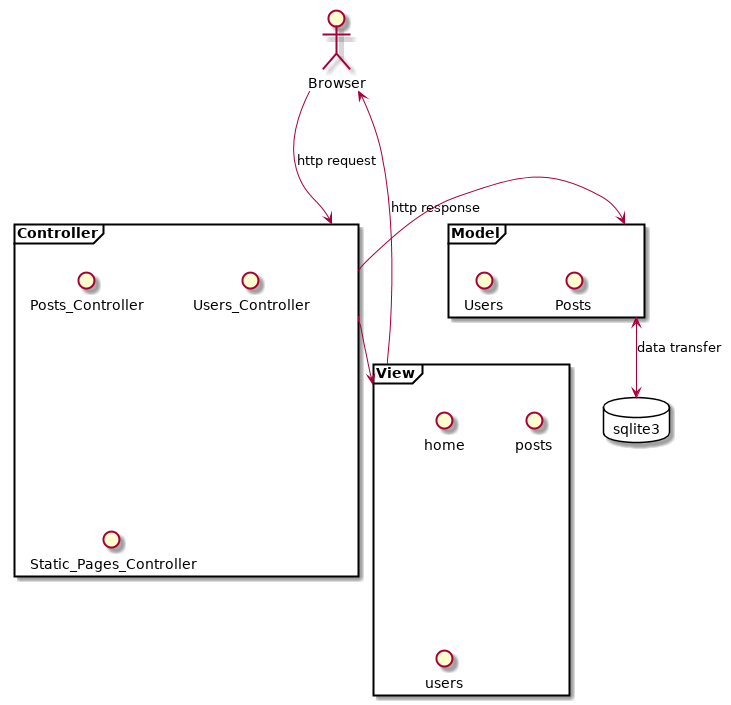
\includegraphics[width=10cm]{classdesign.png}
\caption{\label{fig:classuml}Posts and Users UML}
\end{figure}
\end{center}


\subsubsection{Database}
\label{sec-2-1-2}
\begin{center}
\begin{figure}[htb]
\centering
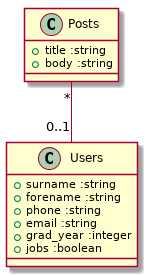
\includegraphics[width=3cm]{posts-users.png}
\caption{\label{fig:userposts}Posts and Users UML}
\end{figure}
\end{center}

\subsection{What is the Model-2 Variant}
\label{sec-2-2}
The model-2 variant of the model view controller, design pattern is one designed for 
medium-large web-based applications \cite{Model1an89:online}.

In this arch-type the server acts as the controller, the view is much more separated and independent
from the controller, than MVC model 1. This makes it much easier to extend the application without
having decentralised components lagging behind and causing issues \cite{javaWhat73:online}. 

\section{Disclaimer}
\label{sec-3}
Covering image used sourced from \url{https://www.ruby-lang.org} \cite{RubyProg39:online}. Diagrams 
made by myself. 

Additionally I acknowledge that all information present in this document is my own work using knowledge
gained from \cite{RubyonRa5:online,RubyProg39:online,javaWhat73:online,loftus17_requir_cs_alumn_applic,Model1an89:online}.

\bibliographystyle{unsrt}
\bibliography{assignment1}
% Emacs 25.3.1 (Org mode 8.2.10)
\end{document}